\documentclass[a4paper, oneside, dvipsnames, table]{article}
\usepackage{../../Utilita/Stiletemplate}
\usepackage{hyperref}
\usepackage{eurosym}
\usepackage{fancyhdr}
\usepackage[italian]{babel}
\usepackage{pdflscape}
\usepackage[raggedright]{titlesec}
\usepackage{blindtext}
\usepackage{pgf-pie}
\usepackage{pgfplots}
\pgfplotsset{compat=1.3}
\titleformat{\paragraph}[hang]{\normalfont\normalsize\bfseries}{\theparagraph}{1em}{}
\titlespacing*{\paragraph}{0pt}{3.25ex plus 1ex minus .2ex}{0.5em}
\newcommand{\ColonnaIstogramma}[8]{(Christian, #1) (Davide, #2) (Emanuele, #3) (Enrico, #4) (Federico, #5) (Francesco, #6) (Riccardo, #7) (Tommaso, #8)}

\newcommand{\Titolo}{Piano di Qualifica}

\newcommand{\Redattori}{\AT{} \newline \MC{} \newline \BR{}}

\newcommand{\Verificatori}{\LD{} \newline \DF{}}

\newcommand{\Approvatore}{\SE{}}

\newcommand{\Distribuzione}{\Proponente{} \newline \VT{} \newline \CR{} \newline Gruppo \Gruppo{}}

\newcommand{\Uso}{Esterno}

\newcommand{\DescrizioneDoc}{Questo documento si occupa di descrivere il \PdQ{} realizzato dal Gruppo \Gruppo{} per il progetto \NomeProgetto{}.}

\newcommand{\pathimg}{../../Utilita/Immagini/qbteam.png}

\newcommand{\Versionedoc}{2.0.0}
% scritto da \DF{},\AT{}

% info generali 
\newcommand{\NomeProgetto}{\textit{Stalker}}

% fornitore
\newcommand{\Gruppo}{\textit{qbteam}}
\newcommand{\Mail}{qbteamswe@gmail.com}
% \newcommand{\pathimg}{Immagini/qbteam.png}

% committenti
\newcommand{\Committente}{\VT \newline \CR}
\newcommand{\VT}{Prof. Vardanega Tullio}
\newcommand{\CR}{Prof. Cardin Riccardo}

% proponenti
\newcommand{\Proponente}{\textit{Imola Informatica}}
\newcommand{\ZD}{Zanetti Davide}
\newcommand{\CT}{Cardona Tommaso}

% qbteam
\newcommand{\AT}{Azzalin Tommaso}
\newcommand{\DF}{Drago Francesco}
\newcommand{\BR}{Baratin Riccardo}
\newcommand{\MC}{Mattei Christian}
\newcommand{\PF}{Perin Federico}
\newcommand{\CE}{Cisotto Emanuele}
\newcommand{\SE}{Salmaso Enrico}
\newcommand{\LD}{Lazzaro Davide}

% ruoli
\newcommand{\Responsabile}{Responsabile di Progetto}
\newcommand{\Amministratore}{Amministratore di Progetto}

% documenti

\newcommand{\SdF}{Studio di Fattibilità}
\newcommand{\SdFv}[1]{\textit{Studio di Fattibilità {#1}}}
\newcommand{\PdQ}{Piano di Qualifica}
\newcommand{\PdQv}[1]{\textit{Piano di Qualifica {#1}}}
\newcommand{\PdP}{Piano di Progetto}
\newcommand{\PdPv}[1]{\textit{Piano di Progetto {#1}}}
\newcommand{\NdP}{Norme di Progetto}
\newcommand{\NdPv}[1]{\textit{Norme di Progetto {#1}}}
\newcommand{\AdR}{Analisi dei Requisiti}
\newcommand{\AdRv}[1]{\textit{Analisi dei Requisiti {#1}}}
\newcommand{\Glossario}{Glossario}
\newcommand{\Glossariov}[1]{\textit{Glossario {#1}}}
\newcommand{\MM}{Manuale Manutentore}
\newcommand{\MU}{Manuale Utente}

% comandi generali
\newcommand{\glo}[1]{#1\ap{G}}

\setlength{\parindent}{-0.1em}


\begin{document}

\copertina{}
\newpage


\fancydoc{}

\section*{Registro delle modifiche}
{
\rowcolors{2}{grigetto}{white}
\renewcommand{\arraystretch}{1.5}
\centering
\begin{longtable}{ c c  C{2.3cm} c C{3cm} C{3.2cm}}
\rowcolor{rossoep}
\textcolor{white}{\textbf{Versione}} & \textcolor{white}{\textbf{Data}} & \textcolor{white}{\textbf{Nominativo}} & \textcolor{white}{\textbf{Ruolo}} & 
\textcolor{white}{\textbf{Verificatore}}& \textcolor{white}{\textbf{Descrizione}}\\	


1.0.0 & \Data & \CE{} & Responsabili & \CE{} & Approvazione per il rilascio.  \\
		
0.0.1 & \Data & \DF{} & Analista & \AT{} & Stesura e verifica del documento.  \\
		
		
\end{longtable}
}


\clearpage
\tableofcontents
\clearpage

\setcounter{table}{0}

\renewcommand{\listtablename}{Elenco tabelle}
\renewcommand{\listfigurename}{Elenco diagrammi}

\listoffigures
\clearpage
\listoftables
\clearpage

% scritto da\AT{}
\section{Introduzione}
\subsection{Scopo del documento}
Il presente documento ha lo scopo di descrivere le strategie che il gruppo \Gruppo{} intende applicare per garantire la qualità di processo e di prodotto per l’intera durata del progetto.
Al fine di rispettare questi obiettivi vengono descritte le modalità in cui vengono effettuate la verifica e la validazione del prodotto.
In questo modo è consentita la rilevazione e correzione di problemi o incongruenze in breve tempo, senza correre il rischio di sprechi di risorse.

\subsection{Scopo generale del prodotto}
L'obiettivo del prodotto \NomeProgetto{} di \Proponente{} è la creazione di un sistema software composto di un applicativo per cellulare e di un server, con cui interagire tramite un'interfaccia utente. La necessità nasce dal bisogno di adempiere alle normative vigenti in tema di sicurezza.
Le due componenti del sistema software, applicativo e server, devono soddisfare i seguenti obiettivi rispettivamente di:
\begin{itemize}
\item Tracciare e registrare i \glo{movimenti} di un utente in un \glo{luogo di tracciamento} di un'\glo{organizzazione}, siano essi autenticati da credenziali di un'\glo{organizzazione} oppure visitatori anonimi, il tutto nel rispetto della normativa sulla privacy;
\item Poter visionare gli accessi degli utenti autenticati e visionare il numero di visitatori anonimi all'interno di un luogo.
\end{itemize}

\subsection{Glossario}
Al fine di evitare ambiguità fra i termini, e per avere chiare fra tutti gli stakeholder le terminologie utilizzate per la realizzazione del presente documento, il gruppo \Gruppo{} ha redatto un documento denominato \Glossariov{1.0.0}.
In tale documento, sono presenti tutti i termini tecnici, ambigui, specifici del progetto e scelti dai membri del gruppo con le loro relative definizioni.
Un termine presente nel \Glossariov{1.0.0} e utilizzato in questo documento viene indicato con un apice \ap{G} alla fine della parola.

\subsection{Standard di progetto}
Il gruppo \Gruppo{} ha deciso di gestire i propri processi del ciclo di vita del software adottando alcune parti dello standard \textbf{ISO/IEC 12207} come definito nelle \textit{NormeDiProgetto}; 
come modello di qualità del prodotto software si è utilizzato parte dello standard \textbf{ISO/IEC 9126} anch'esso definito nelle \textit{NormeDiProgetto}.

\subsection{Riferimenti}

\subsubsection{Normativi}
\begin{itemize}
    \item \textbf{Capitolato d'appalto C5 - Stalker}\\     
    \url{https://www.math.unipd.it/~tullio/IS-1/2019/Progetto/C5.pdf};
    \item \NdPv{1.0.0}.
    \item \textbf{ISO/IEC 12207-1995:}\\     
    \url{https://www.math.unipd.it/~tullio/IS-1/2009/Approfondimenti/ISO_12207-1995.pdf};\\
    \url{http://www.colonese.it/SviluppoSw_Standard_ISO12207.html};
    \item \textbf{ISO/IEC 9126:}\\
    \url{http://www.colonese.it/00-Manuali_Pubblicatii/07-ISO-IEC9126_v2.pdf};\\
    \url{https://en.wikipedia.org/wiki/ISO/IEC_9126};
\end{itemize}

\subsubsection{Informativi}
\begin{itemize}
    \item \textbf{Indice di Gulpease}\\
    \url{https://it.wikipedia.org/wiki/Indice_Gulpease};
    \item \textbf{Metriche di progetto}\\
    \url{https://it.wikipedia.org/wiki/Metriche_di_progetto};
    \item \textbf{Varie metriche}\\
    \url{http://torlone.dia.uniroma3.it/sistelab/annipassati/sbavaglia.pdf};
    \item \textbf{Ciclo di Deming - Plan Do Check Act}\\
    \url{https://it.wikipedia.org/wiki/Ciclo_di_Deming};
    
\end{itemize}
\clearpage
\section{Analisi dei Rischi}
La gestione dei rischi è un processo al quale il gruppo \Gruppo{} dà molto importanza. Questo perché incorrere in rischio potrebbe equivalere al danneggiamento del progetto, sia nella sua organizzazione\ap{G} e sia nella sua qualità.
Si cerca quindi di fare una previsione dei problemi che si potrebbero verificare durante l'intero corso del progetto e, per ogni rischio identificato, si cerca una soluzione per poterlo evitare.

\subsection{Fasi della gestione dei rischi}
Il gruppo seguirà i seguenti step del processo di gestione dei rischi:
\begin{itemize}
	\item \textbf{Identificazione del rischio}: Questo è il primo step del processo e ci serve per identificare i rischi che potrebbero portare a dei problemi durante l'avanzamento del progetto; 
\end{itemize}
\begin{itemize}
	\item \textbf{Analisi dei rischi}: Dopo aver individuato i rischi nello step precedente, per ognuno di essi si valuterà la probabilità che si verifichi e le conseguenze negative che potrebbe portare;
\end{itemize}
\begin{itemize}
	\item \textbf{Pianificazione del rischio}: Nella pianificazione del rischio si sviluppano dei piani per sapere quali rimedi bisognerà intraprendere nel momento in cui i rischi si verificano. In tale maniera si riuscirà a risolvere i problemi prima che essi si aggravino;
\end{itemize}
\begin{itemize}
	\item \textbf{Monitoraggio del rischio}: Nell'ultimo step della gestione del rischio si verifica che le ipotesi relative ai rischi non abbiano subito delle variazioni. Quindi si cerca di valutare periodicamente la probabilità che il rischio si verifichi e i suoi possibili effetti migliorando le strategie adottate per la loro risoluzione.
\end{itemize}

\subsection{Tipologia del rischio}
Ci sono 5 tipi di rischi che il gruppo \Gruppo{} terrà in considerazione. 
\\Ad ogni rischio verrà assegnato un codice identificativo:
\begin{itemize}
	\item Rischi Tecnologici [RT];
	\item Rischi Organizzativi [RO];
	\item Rischi Personali [RP];
	\item Rischi dei Requisiti [RR];
	\item Rischi di Stima [RS].
\end{itemize}

\subsection{Tabella dei rischi}
Nella seguente tabella verranno elencati i rischi che il gruppo \Gruppo{} potrebbe incontrare durante l'intero ciclo di vita del progetto.
Ogni colonna di un rischio sarà composto da:
\begin{itemize}
	\item Codice [codice del tipo + numero sequenziale] e Nome del Rischio;
	\item Descrizione;
	\item Rilevamento;
	\item Piano di Contingenza.
\end{itemize}



\clearpage
\section{Modello di Sviluppo}
Come modello di sviluppo il gruppo \Gruppo{} ha deciso di adottare il \textbf{modello incrementale}.
\subsection{Descrizione}
Nel modello incrementale il prodotto viene sviluppato tramite rilasci successivi. Questi rilasci hanno l'obiettivo di aggiungere funzionalità separate e accessorie a un sistema stabile in cui sono presenti requisiti di base.
Nel caso in cui un rilascio sia fallace è molto facile tornare allo stato funzionante precedente.\\
Il modello incrementale richiede, dunque, una suddivisione preliminare dei requisiti atta ad identificare quelli da sviluppare per primi e quali aggiungere al sistema stabile per incrementi. \\
Inoltre, una volta implementate le caratteristiche base del sistema lo si può sottoporre al committente e al proponente per assicurarsi di star procedendo nella giusta direzione.
In caso negativo, non è troppo tardi per cambiare la struttura del prodotto corrente. \\
Infine, non è particolarmente dispendioso riformulare degli incrementi previsti ma che devono ancora essere implementati. 

\subsection{Motivazioni}
Il gruppo ha scelto questo modello di sviluppo perché si adatta bene alle specifiche del progetto \NomeProgetto{} del proponente \Proponente{}.
Nella fattispecie, è stato facile identificare i requisiti minimi e separare molti requisiti accessori perfetti per essere implementati tramite rilasci incrementali su di un sistema stabile.\\
Inoltre, data la nostra inesperienza, il modello scelto permette a eventuali cambiamenti in corso d'opera di essere poco dispendiosi dal punto di vista sia del tempo di codifica (se circoscritti a singoli rilasci), sia del lavoro di cambiamento della documentazione. \\
In aggiunta a ciò, i rilasci successivi di funzionalità permettono di poter stabilire un confronto migliore con il proponente, riuscendo a sottoporre al suo giudizio un prodotto che sia sempre funzionante e col tempo sempre più completo e conforme alle sue aspettative. \\
Abbiamo inoltre valutato che i principali difetti del modello incrementale, quali la degradazione della struttura causata dall'aggiunta di incrementi e l'invisibilità del processo al manager, 
non influenzano il gruppo data la dimensione ridotta, relativamente ad ambienti aziendali dove i modelli di sviluppo sono sfruttati a pieno, del progetto che stiamo affrontando.


\subsection{Individuazione degli incrementi}
In seguito è riportata una tabella con indicati i requisiti che vengono sviluppati in ciascun incremento, sia dell'applicazione che del server.
I requisiti sono identificati dal loro codice identificativo e sono reperibili nel documento \AdR{}.\\
I codici dei requisiti enfatizzati in grassetto sono obbligatori, quelli non evidenziati sono requisiti desiderabili oppure opzionali.
La scelta di enfatizzare quelli grafici è puramente per una maggior comodità di consultazione.

{
\rowcolors{2}{grigetto}{white}
\renewcommand{\arraystretch}{2}
\centering
	
\begin{longtable}{C{2.5cm} C{3.2cm} C{2.8cm} C{2.8cm} C{2.8cm}}
\caption{Tabella degli incrementi}\\
\rowcolor{darkblue}
\textcolor{white}{\textbf{Incremento}} &
\textcolor{white}{\textbf{Obiettivo dell'incremento}} & 
\textcolor{white}{\textbf{Requisiti per l'app utenti}} &
\textcolor{white}{\textbf{Requisiti per il web-app admin}} &
\textcolor{white}{\textbf{Requisiti per il server}} \\
\endhead

Incremento 0 & \glo{Proof of Concept} (app utenti e web-app admin), lista delle organizzazioni e tracciamento (app utenti, web-app admin, server) (a livello dimostrativo per il \glo{Proof of Concept}) & \begin{itemize}
    % APP
    \item[ ] R1FI1
    \item[ ] R1FA1.1
    \item[ ] R1FA1.2
    \item[ ] R1FA1.3
    \item[ ] R1FA1.4
    \item[ ] R1FA1.5
    \item[ ] R1FA2.1
    \item[ ] R1FA3.1
    \item[ ] R1FA3.8
    \item[ ] R1FA3.10
    \item[ ] R1FA6.1
    \item[ ] R1FA8.1
    \item[ ] R1FA8.4
\end{itemize} & \begin{itemize}
    % WEB-APP ADMIN
    \item[ ] R1FI2
    \item[ ] R1FS1.1
    \item[ ] R1FS1.2
    \item[ ] R2FS1.3
    \item[ ] R2FS1.4
    \item[ ] R2FS1.5
    \item[ ] R2FS1.6
    \item[ ] R2FS1.7
    \item[ ] R1FS2.1
    \item[ ] R1FS3.1
    \item[ ] R1FS6.1
    \item[ ] R1FS10.1
    \item[ ] R1FS10.2
    \item[ ] R1FS10.14
\end{itemize} & \begin{itemize} 
    % SERVER
    \item[ ] R1FS3.1
    \item[ ] R1FI5
    \item[ ] R2FI7
    \item[ ] R1FI8
    \item[ ] R1FA3.2
    \item[ ] R1FA6.1

\end{itemize}\\

Incremento 1 & Funzionalità di autenticazione (app utenti e web-app admin) & \begin{itemize}
    % APP
    \item[ ] R1FI1
    \item[ ] R1FA1.1
    \item[ ] R1FA1.2
    \item[ ] R1FA1.3
    \item[ ] R1FA1.4
    \item[ ] R1FA1.5
    \item[ ] R1FA1.6
    \item[ ] R1FA1.7
    \item[ ] R1FA2.1
    \item[ ] R1FA8.1
    \item[ ] R1FA8.2
    \item[ ] R1FA8.3
    \item[ ] R1FA8.4
\end{itemize} & \begin{itemize}
    % WEB-APP ADMIN
    \item[ ] R1FI2
    \item[ ] R1FS1.1
    \item[ ] R1FS1.2
    \item[ ] R1FS2.1
    \item[ ] R1FS10.1
    \item[ ] R1FS10.2
\end{itemize} & 
    % SERVER
    Nessun requisito del server previsto per questo incremento \\

Incremento 2 & Lista delle organizzazioni (app utenti e web-app admin) & \begin{itemize}
    % APP
    \item[ ] R1FA3.1
    \item[ ] R1FA3.2
    \item[ ] R1FA3.3
    \item[ ] R1FA3.4
    \item[ ] R1FA3.5
    \item[ ] R1FA3.6
    \item[ ] R1FA3.7
    \item[ ] R1FA3.8
    \item[ ] R1FA3.9
    \item[ ] R1FA3.10
    \item[ ] R1FA3.15
    \item[ ] R1FA3.17
    \item[ ] R1FA8.5
    \item[ ] R1FA8.6
\end{itemize} & \begin{itemize} 
    % WEB-APP ADMIN
    \item[ ] R1FC3
    \item[ ] R1FI3
    \item[ ] R1FI5
    \item[ ] R1FI8
    \item[ ] R1FS3.1
    \item[ ] R1FS7.1
    \item[ ] R1FS7.2
    \item[ ] R1FS7.6
\end{itemize} & \begin{itemize} 
    % SERVER
    \item[ ] R1FC3
    \item[ ] R1FI3
    \item[ ] R1FI8
    \item[ ] R1FS3.1
    \item[ ] R1FS7.1
    \item[ ] R1FS7.2
    \item[ ] R1FS7.6
\end{itemize}\\

Incremento 3 & Tracciamento & \begin{itemize}
    % APP
    \item[ ] R1FA4.1
    \item[ ] R1FA4.2
    \item[ ] R1FA4.3
    \item[ ] R1FA6.1
    \item[ ] R1FA6.2
    \item[ ] R1FA6.3
    \item[ ] R1FA6.4
    \item[ ] R1FA8.7
    \item[ ] R1FA7.1
    \item[ ] R1FA8.8
    \item[ ] R1FA7.2
    \item[ ] R1FA7.3
\end{itemize}& \begin{itemize} 
    % WEB-APP ADMIN
    \item[ ] R1FS6.1
    \item[ ] R1FS6.2
    \item[ ] R1FS6.3
    \item[ ] R1FS8.1
    \item[ ] R1FS8.2
    \item[ ] R1FS8.3
    \item[ ] R1FS8.4

\end{itemize} & \begin{itemize} 
    % SERVER 
    \item[ ] R1FA6.1
    \item[ ] R1FA6.2
    \item[ ] R1FA6.3
    \item[ ] R1FA6.4
    \item[ ] R1FA8.7
    \item[ ] R1FS6.1
    \item[ ] R1FS6.2
    \item[ ] R1FS8.1
    \item[ ] R1FS8.2
    \item[ ] R1FS8.3
    \item[ ] R1FS8.4
\end{itemize}\\

Incremento 4 & Storico accessi di un utente (app utenti) e report tabellari degli accessi (web-app admin) &
    % APP
    Nessun requisito dell'applicazione previsto per questo incremento
    & \begin{itemize} 
    % WEB-APP ADMIN
    \item[ ] R1FS4.1
    \item[ ] R1FS4.4
    \item[ ] R1FS4.5
    \item[ ] R1FS4.6
    \item[ ] R1FS4.8
    \item[ ] R1FS10.3
    \item[ ] R1FS10.4
    \item[ ] R1FS10.7
    \item[ ] R1FS10.8
    \item[ ] R1FS5.1
    \item[ ] R1FS10.9
    \item[ ] R1FS5.2
    \item[ ] R1FS5.9
    \item[ ] R1FS5.3
    \item[ ] R1FS10.10
    \item[ ] R1FS5.4
    \item[ ] R1FS5.5
    \item[ ] R1FS5.6
    \item[ ] R2FS5.7
    \item[ ] R1FS5.8
\end{itemize} & \begin{itemize} 
    % SERVER
    \item[ ] R1FS4.1
    \item[ ] R1FS4.4
    \item[ ] R1FS4.5
    \item[ ] R1FS4.6
    \item[ ] R1FS4.8
    \item[ ] R1FS10.3
    \item[ ] R1FS10.4
    \item[ ] R1FS10.7
    \item[ ] R1FS10.8
    \item[ ] R1FS5.1
    \item[ ] R1FS10.9
    \item[ ] R1FS5.2
    \item[ ] R1FS5.9
    \item[ ] R1FS5.3
    \item[ ] R1FS10.10
    \item[ ] R1FS5.4
    \item[ ] R1FS5.5
    \item[ ] R1FS5.6
    \item[ ] R2FS5.7
    \item[ ] R1FS5.8
\end{itemize} \\

Incremento 5 & Autenticazione presso l'organizzazione (app utenti), gestione amministratori  e modifica dell'organizzazione (web-app admin) & \begin{itemize}
    % APP
    \item[ ] R1FS9.12
    \item[ ] R1FS9.13
    \item[ ] R1FS9.14
\end{itemize} & \begin{itemize} 
    % WEB-APP ADMIN
    \item[ ] R1FI9
    \item[ ] R1FI10
    \item[ ] R1FI11
    \item[ ] R1FS9.1
    \item[ ] R1FS9.2
    \item[ ] R1FS9.3
    \item[ ] R1FS9.4
    \item[ ] R1FS9.5
    \item[ ] R1FS9.6
    \item[ ] R1FS9.7
    \item[ ] R1FS9.8
    \item[ ] R1FS9.9
    \item[ ] R1FS9.10
    \item[ ] R1FS9.11
    \item[ ] R1FS9.12
    \item[ ] R1FS9.13
    \item[ ] R1FS9.14
    \item[ ] R1FS10.11
    \item[ ] R1FS10.12
    \item[ ] R1FS10.13
    \item[ ] R1FS10.14
    \item[ ] R1FS10.15
    \item[ ] R1FS10.16
    \item[ ] R1FS10.17
\end{itemize} & \begin{itemize}
    % SERVER
    \item[ ] R1FI9
    \item[ ] R1FI10
    \item[ ] R1FI11
    \item[ ] R1FS9.2
    \item[ ] R1FS9.3
    \item[ ] R1FS9.4
    \item[ ] R1FS9.6
    \item[ ] R1FS9.7
    \item[ ] R1FS9.8
    \item[ ] R1FS9.9
    \item[ ] R1FS9.10
    \item[ ] R1FS9.12
    \item[ ] R1FS9.13
    \item[ ] R1FS10.11
    \item[ ] R1FS10.12
    \item[ ] R1FS10.14
    \item[ ] R1FS9.14
    \item[ ] R1FS10.15
\end{itemize}\\

Incremento 6 & Funzionalità aggiuntive all'utente anonimo & \begin{itemize}
    % APP
    \item[ ] R2FA5.1
    \item[ ] R2FA5.2
    \item[ ] R2FA5.3
    \item[ ] R2FA5.4
    \item[ ] R2FA5.5
    \item[ ] R2FA5.6
    \item[ ] R2FA5.7
    \item[ ] R2FA5.8
    \item[ ] R2FA5.9
    \item[ ] R2FA5.10
    \item[ ] R2FA5.11
    \item[ ] R3FA5.12
    \item[ ] R2FA5.13
    \item[ ] R2FA5.14
    \item[ ] R3FA5.15
    \item[ ] R2FA5.16
    \item[ ] R2FA5.17
    \item[ ] R2FA8.5
    \item[ ] R2FA8.6
\end{itemize} &
    % WEB-APP ADMIN
    Nessun requisito della web-app admin previsto per questo incremento
    & \begin{itemize} 
    % SERVER
    \item[ ] R2FA5.1
    \item[ ] R2FA5.2
    \item[ ] R2FA5.3
    \item[ ] R2FA5.4
    \item[ ] R2FA5.5
    \item[ ] R2FA5.6
    \item[ ] R2FA5.7
    \item[ ] R2FA5.8
    \item[ ] R2FA5.9
    \item[ ] R2FA5.16
    \item[ ] R2FA5.17
    \item[ ] R2FA8.5
    \item[ ] R2FA8.6
\end{itemize}\\

Incremento 7 & Funzionalità per il reset della password & \begin{itemize}
    % APP
    \item[ ] R2FA1.8
    \item[ ] R2FA1.9
    \item[ ] R2FA1.10
    \item[ ] R2FA1.11
    \item[ ] R2FA1.12
\end{itemize} & \begin{itemize} 
    % WEB-APP ADMIN
    \item[ ] R2FS1.3 %poc
    \item[ ] R2FS1.4 %poc
    \item[ ] R2FS1.5 %poc
    \item[ ] R2FS1.6 %poc
    \item[ ] R2FS1.7 %poc
\end{itemize} & 
    % SERVER
    Nessun requisito del server previsto per questo incremento \\

Incremento 8 & Funzionalità aggiuntive di filtraggio/ricerca nella lista delle organizzazioni (app utenti e web-app admin) & \begin{itemize}
    % APP
    \item[ ] R2FA3.11
    \item[ ] R2FA3.12
    \item[ ] R3FA3.13
    \item[ ] R3FA3.14
    \item[ ] R2FA3.16
    \item[ ] R2FA3.18
\end{itemize} & \begin{itemize} 
    % WEB-APP ADMIN
    \item[ ] R2FI4
    \item[ ] R2FI6
    \item[ ] R2FI7
    \item[ ] R2FS7.3
    \item[ ] R2FS7.4
    \item[ ] R2FS7.5
    \item[ ] R2FS7.7 
    \item[ ] R2FS7.8 
    \item[ ] R2FS7.9
\end{itemize} & \begin{itemize} 
    % SERVER
    \item[ ] R2FI4
    \item[ ] R2FI6
    \item[ ] R2FI7
\end{itemize}\\

Incremento 9 & Funzionalità generiche aggiuntive agli amministratori e gestione errori & 
    % APP
    Nessun requisito dell'app previsto per questo incremento
     & \begin{itemize} 
    % WEB-APP ADMIN
    \item[ ] R2FS4.2
    \item[ ] R2FS4.3
    \item[ ] R3FS4.7
    \item[ ] R2FS10.5
    \item[ ] R2FS10.6
    \item[ ] R2FS10.18
\end{itemize} & \begin{itemize} 
    % SERVER
    \item[ ] R2FS4.2
    \item[ ] R2FS4.3
    \item[ ] R3FS4.7
    \item[ ] R2FS10.5
    \item[ ] R2FS10.6
    \item[ ] R2FS10.18
\end{itemize} \\

\end{longtable}
}
\clearpage
\section{Pianificazione}
Nella pianificazione, il responsabile suddividerà il lavoro in attività e le assegnerà a ciascun membro del team.
Lo scopo è quello di mostrare come verrà svolto il lavoro, valutare i progressi nel progetto e anticipare i problemi che potrebbero sorgere preparando così delle soluzioni a tali problemi. 
La pianificazione di progetto è stata organizzata seguendo le scadenze presenti nella sezione § 8.1 Scadenze.
Lo sviluppo del progetto è stato suddiviso nelle seguenti 4 fasi: 
\begin{itemize}
	\item Analisi;
	\item Progettazione Architetturale;
	\item Progettazione di Dettaglio e Codifica;
	\item Validazione e Collaudo;
\end{itemize}
Ogni fase sarà suddivisa in periodi più brevi all'interno dei quali verranno elencate le diverse attività che il gruppo \Gruppo{} svolgerà.


\subsection{Analisi}

\subsubsection{Periodo 1} 
Dal 2019-11-15 al 2019-11-29\\
In questo periodo, che parte dalla formazione del gruppo e termina con la scelta del capitolato C5, abbiamo affrontato le seguenti tematiche al fine di porre le basi per il lavoro che dovevamo affrontare:\\
\begin{itemize}
	\item \textbf{Discussione capitolati:} per prima cosa abbiamo studiato individualmente e in seguito discusso durante gli incontri tutti i capitolati proposti, questo ha posto le basi per la stesura del documento \SdF{} e ci ha indirizzati verso la scelta del capitolato che avremmo affrontato;
	\item \textbf{Spartizione e studio dei ruoli:} a ogni membro del gruppo è stato assegnato il ruolo che svolgerà nella fase di Analisi;
	\item \textbf{Definizione degli strumenti:} Abbiamo discusso e definito le tecnologie che avremmo usato per affrontare la fase di Analisi;
	\item \textbf{Pianificazione milestone fase di Analisi:} Abbiamo discusso e fissato delle milestone da rispettare per completare la fase di Analisi entro le scadenze imposteci.
\end{itemize}
\subsubsection{Periodo 2} 
Dal 2019-11-30 al 2019-12-31\\
Questo periodo inizia con la scelta definitiva del capitolato C5.\\
Dopo la scelta abbiamo focalizzato le risorse del gruppo sui seguenti punti:
\begin{itemize}
	\item \textbf{Normazione: }Abbiamo definito le regole per la stesura dei documenti e per l'utilizzo delle tecnologie identificate in precedenza;
	\item \textbf{Approfondimento capitolati: }Abbiamo ulteriormente discusso tutti i capitolati in modo da terminare lo studio di fattibilità e focalizzato la nostra analisi su quello scelto in modo da predisporre le basi per l'analisi dei requisiti;
	\item \textbf{Prima definizione dei casi d'uso};
	\item \textbf{Determinazione standard di qualità: }Abbiamo definito le nostre strategie per garantire la qualità di processo e di prodotto;
	\item \textbf{Verifica: }Verifica dell'andamento del team in relazione alle tempistiche e allo svolgimento dei compiti assegnati.
\end{itemize}
\subsubsection{Periodo 3}
 Dal 2020-01-01 al 2020-01-14\\
 Questo periodo si estende fino alla data ultima di consegna per affrontare la revisione dei requisiti a cui il nostro gruppo ha deciso di partecipare.\\
 \begin{itemize}
	\item \textbf{Normazione: }Ulteriori approfondimenti alle regole per la stesura dei documenti e per l'utilizzo delle tecnologie;
	\item \textbf{Approfondimento delle tecnologie: }Abbiamo ampliato le nostre conoscenze sulle tecnologie richieste dal capitolato per essere svolto;
	\item \textbf{Analisi dei requisiti: } Studio dei requisiti e raffinamento dei casi d'uso;
	\item \textbf{Pianificazione attività: }Pianificazione del lavoro da svolgere nelle fasi successive a quella di Analisi;
	\item \textbf{Verifica: }Verifica dell'andamento del team in relazione alle tempistiche e allo svolgimento dei compiti assegnati.

 \end{itemize}
\subsubsection{Periodo 4} 
Dal 2020-01-15 al 2020-01-20\\
In questo periodo che parte dalla consegna dei documenti per la revisione dei requisiti alla presentazione pubblica della proposta il gruppo consolida il lavoro svolto in vista delle successive fasi e della discussione per la quale serve una presentazione;
\begin{itemize}
	\item \textbf{Consolidamento:} Ogni membro si prende del tempo per ripassare tutto il lavoro svolto e per studiare il necessario per affrontare al meglio le fasi successive;
	\item \textbf{Preparazione per la Revisione dei Requisiti:} Il gruppo produce il materiale necessario da esporre alla presentazione pubblica della nostra proposta.
\end{itemize}

	\newpage
	% Inizia la pagina orientata orizzontalmente
	\begin{landscape}
	 % Ora la pagina e' in orizzontale!
	\subsubsection{Diagramma di Gantt delle attività}
	\pagestyle{empty}
	\begin{figure}[h]
		
		\begin{center}	
			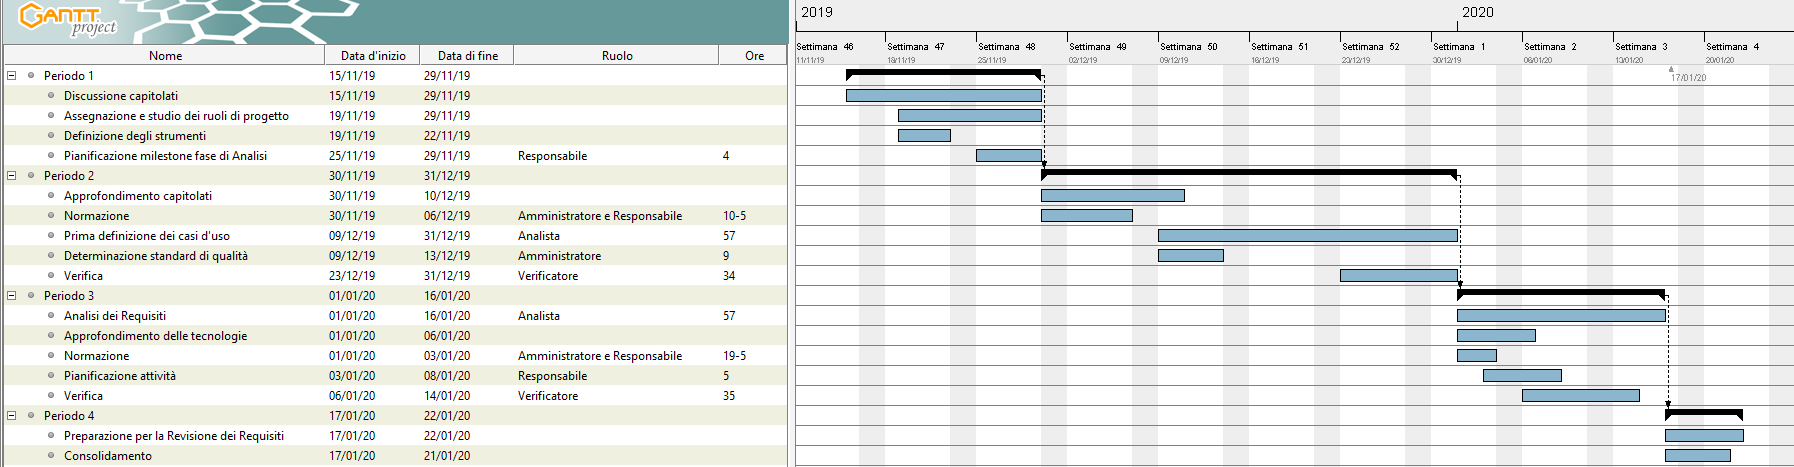
\includegraphics[scale=0.50]{Sezioni/DiagrammiGantt/Analisi.png}
		\end{center}
	\caption{Diagramma di Gantt delle attività di Analisi}
	\end{figure}
	 \end{landscape}

\clearpage
\subsection{Progettazione Architetturale}
Periodo: dal 2020-01-22 al 2020-03-15.
\\Inizia al termine dell'Analisi dei Requisiti e finisce con la data di consegna della Revisione di Progettazione.
\\In questa fase viene definita una soluzione architetturale in modo da soddisfare i requisiti individuati nel periodo di Analisi dei Requisiti.

\subsubsection{Periodo 1} 
Dal 2020-01-22 al 2020-02-11
\begin{itemize}
	\item \textbf{Normazione};
	\item \textbf{Analisi dei requisiti};
	\item \textbf{Pianificazione attività};
	\item \textbf{Approfondimento delle tecnologie};
	\item \textbf{Verifica}.
\end{itemize}
\subsubsection{Periodo 2} 
Dal 2020-02-12 al 2020-03-08
\begin{itemize}
	\item \textbf{Studio delle tecnologie:} IAAS Kubernetes\ap{G} o PaaS\ap{G}, Openshift\ap{G} o Rancher\ap{G}, LDAP\ap{G} e GPS\ap{G};
	\item \textbf{Normazione};
	\item \textbf{Miglioramento standard di qualità};
	\item \textbf{Technology Baseline\ap{G}:} redazione della Technology baseline;
	\item \textbf{Proof of Concept\ap{G}:} rappresentazione della Baseline\ap{G};
	\item \textbf{Codifica:} viene codificato il Proof of Concept;
	\item \textbf{Verifica}.
\end{itemize}
\subsubsection{Periodo 3} 
Dal 2020-03-09 al 2020-03-15
\begin{itemize}
	\item \textbf{Consolidamento};
	\item \textbf{Preparazione per la Revisione di Progettazione Architetturale}.
\end{itemize}

\newpage
% Inizia la pagina orientata orizzontalmente
\begin{landscape}
	% Ora la pagina e' in orizzontale!
	\subsubsection{Diagramma di Gantt delle attività}
	\pagestyle{empty}
	\begin{figure}[h]
		
		\begin{center}	
			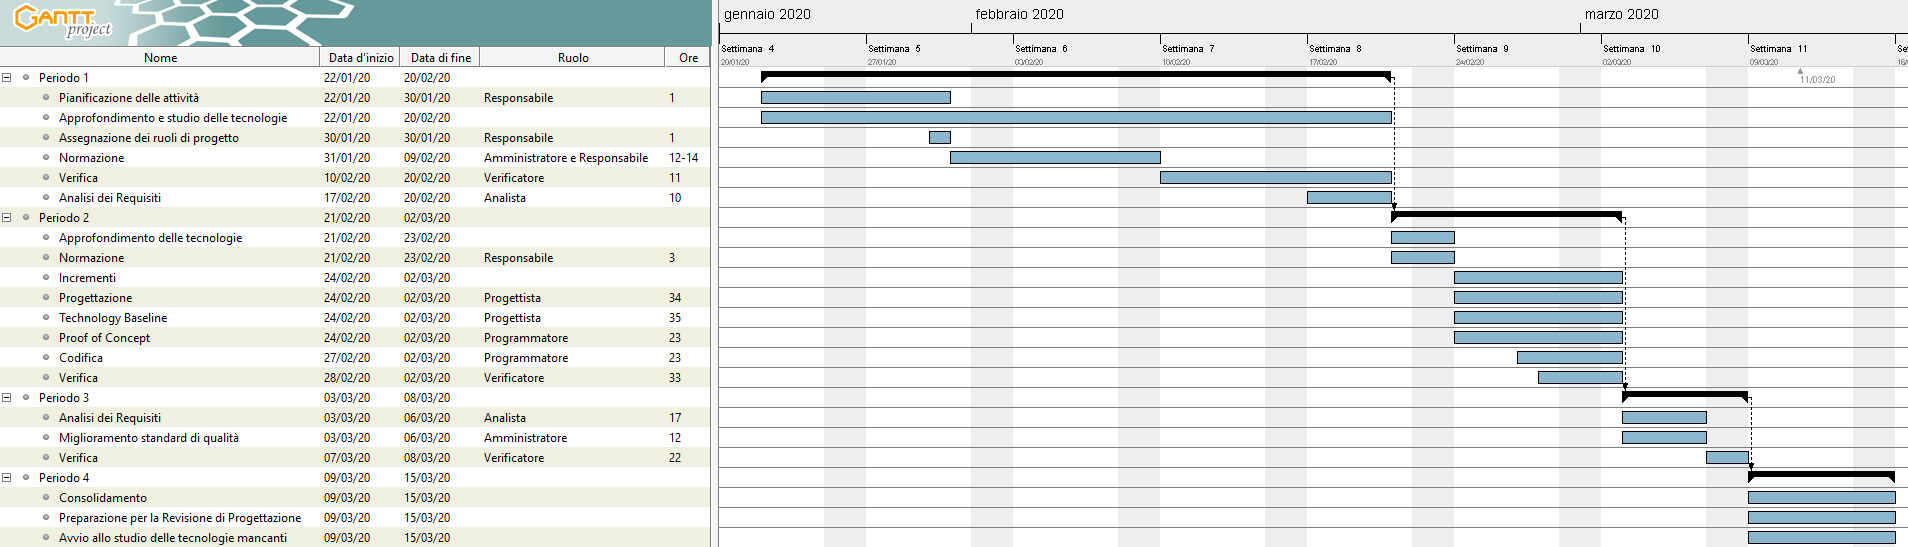
\includegraphics[scale=1.6]{Sezioni/DiagrammiGantt/ProgettazioneArchitetturale.png}
		\end{center}
	\caption{Diagramma di Gantt delle attività di Progettazione}	
	\end{figure}
\end{landscape}

\subsection{Progettazione di Dettaglio e Codifica}
Dal 2020-03-16 al 2020-04-19\\
Inizia al termine della Progettazione Architetturale e finisce con la data di consegna della Revisione di Qualifica.\\
In questa fase si definisce nel dettaglio e si implementa l'architettura logica costruita nella fase di Progettazione Architetturale.\\


\subsubsection{Periodo 1} 
Dal 2020-03-16 al 2020-03-27\\
\begin{itemize}
	\item \textbf{Approfondimento delle tecnologie};
	\item \textbf{Normazione};
	\item \textbf{Pianificazione delle attività};
	\item \textbf{Progettazione};
	\item \textbf{Codifica:} Implementazione dei requisiti di base identificati per ottenere un sistema stabile;
	\item \textbf{Manuali:} Stesura manuale utente e manuale manutentore in relazione alle funzionalità di base del sistema.
\end{itemize}
\subsubsection{Periodo 2} 
Dal 2020-03-28 al 2020-04-08\\
\begin{itemize}
	\item \textbf{Implementazione della Product Baseline:} seguendo le specifiche della Technology Baseline;
	\item \textbf{Codifica incrementale:} Aggiunta di requisiti al sistema tramite incrementi;
	\item \textbf{Incremento e verifica:} Verifiche ed eventuali aggiunte al lavoro svolto in precedenza;
	\item \textbf{Manuali:} Aggiunta nel manuale utente e nel manuale manutentore delle funzionalità inserite incrementalmente nel sistema;
\end{itemize}
\subsubsection{Periodo 3}
Dal 2020-04-09 al 2020-04-12\\
\begin{itemize}
	\item \textbf{Primo rilascio del prodotto};
	\item \textbf{Verifica:} Verifica dell'andamento del team in relazione alle tempistiche e allo svolgimento dei compiti assegnati;
\end{itemize}
\subsubsection{Periodo 4} 
Dal 2020-04-13 al 2020-04-19\\
\begin{itemize}
	\item \textbf{Consolidamento};
	\item \textbf{Preparazione per la Revisione di Qualifica}.
\end{itemize}

\newpage
% Inizia la pagina orientata orizzontalmente
\begin{landscape}
	% Ora la pagina e' in orizzontale!
	\subsubsection{Diagramma di Gantt delle attività}
	\pagestyle{empty}
	\begin{figure}[h]
			
		\begin{center}	
				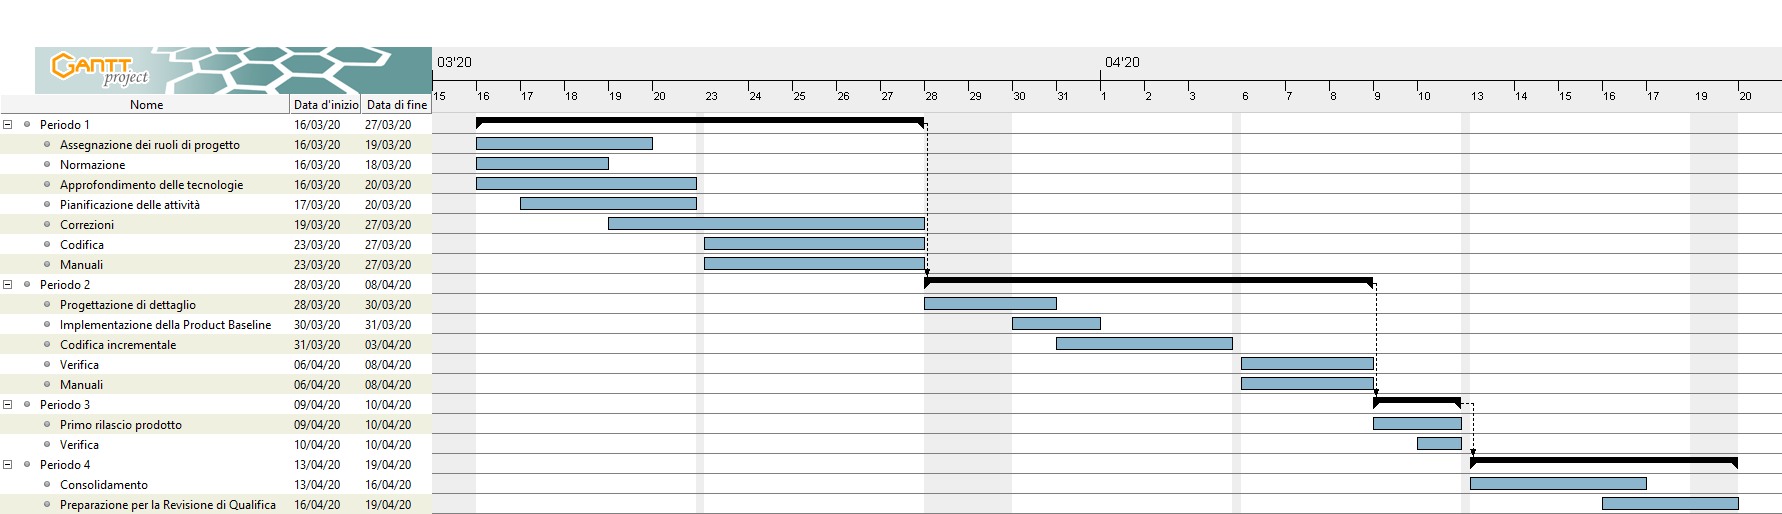
\includegraphics[scale=0.5]{Sezioni/DiagrammiGantt/ProgettazioneDiDettaglio.png}	
		\end{center}
	\caption{Diagramma di Gantt delle attività di Progettazione di Dettaglio e Codifica}	
	\end{figure}
\end{landscape}

\subsection{Validazione e Collaudo}
Inizia al termine della Progettazione di Dettaglio e Codifica e finisce con la data di consegna della Revisione di Accettazione.
\\In questo fase vengono definite le attività che servono per verificare che il prodotto corrisponde a quello desiderato dal cliente.
\subsubsection{Periodo 1} 
Dal 2020-04-21 al 2020-04-28
\begin{itemize}
	\item \textbf{Normazione};
	\item \textbf{Analisi dei requisiti};
	\item \textbf{Pianificazione attività};
	\item \textbf{Verifica}.
\end{itemize}
\subsubsection{Periodo 2} 
Dal 2020-04-29 al 2020-05-10
\begin{itemize}
	\item \textbf{Codifica:} verrà eseguito l'ultimo versionamento del prodotto;
	\item \textbf{Verifica:} verrà accertato che le esecuzioni delle attività siano esenti da errori;
	\item \textbf{Validazione:} verrà verificato se il prodotto realizzato sia conforme alle attese;
	\item \textbf{Scrittura dei manuali:} verrà eseguito il secondo versionamento del manuale Utente e del manuale Manutentore;
	\item \textbf{Collaudo:} vengono eseguiti gli ultimi test sul prodotto per verificare se le funzionalità rispettano i risultati attesi.
\end{itemize}
\subsubsection{Periodo 3} 
Dal 2020-05-11 al 2020-05-17
\begin{itemize}
	\item \textbf{Preparazione per la Revisione di Accettazione}.
\end{itemize}


\newpage
% Inizia la pagina orientata orizzontalmente
\begin{landscape}
	% Ora la pagina e' in orizzontale!
	\subsubsection{Diagramma di Gantt delle attività}
	\pagestyle{empty}
	\begin{figure}[h]
		
		\begin{center}	
			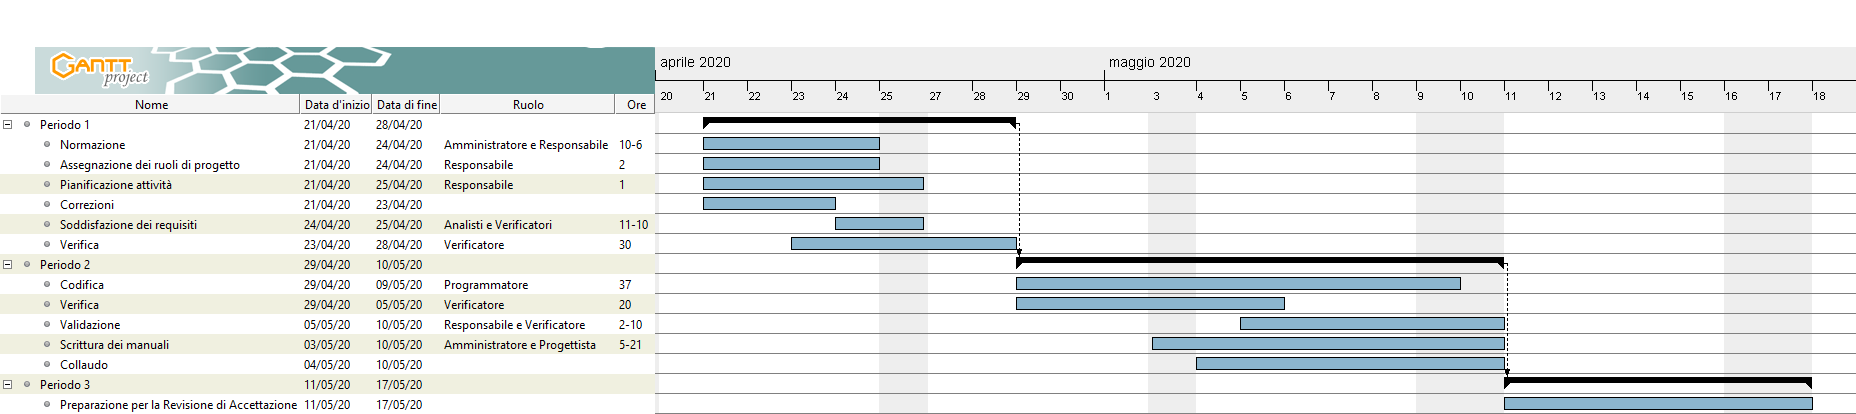
\includegraphics[scale=1.6]{Sezioni/DiagrammiGantt/Validazione.png}
		\end{center}
	\caption{Diagramma di Gantt delle attività di Validazione e Collaudo}	
	\end{figure}
\end{landscape}
\clearpage
\section{Preventivo}
Sigle identificative per i ruoli indicati nelle tabelle e nei grafici:
\begin{itemize}
    \item RE: Responsabile;
    \item AM: Amministratore;
    \item AN: Analista;
    \item PT: Progettista;
    \item PR: Programmatore;
    \item VE: Verificatore.
\end{itemize}
{
	
\rowcolors{2}{grigetto}{white}
\renewcommand{\arraystretch}{2}
\begin{table}[h!]
\centering
\caption{Tabella con i costi per ogni ruolo}
\begin{longtable}{ C{3cm} C{3cm}}
\rowcolor{darkblue}
	\textcolor{white}{\textbf{Ruolo}} & 
	\textcolor{white}{\textbf{Costo per ora espresso in euro}}\\	
			
			Responsabile & 30\\
			Amministratore & 20\\
			Analista & 25\\
			Progettista & 22\\
			Programmatore & 15\\
			Verificatore & 15\\
			
		\end{longtable}
		
	\end{table}

}

\clearpage
\subsection{Fase di Analisi}
\subsubsection{Divisione Oraria}

La seguente tabella rappresenta la distribuzione oraria dei ruoli per ogni componente del gruppo:
\rowcolors{2}{grigetto}{white}
\renewcommand{\arraystretch}{2}
\begin{table}[h!]
\centering
\caption{Tabella della divisione oraria di Analisi}	
\begin{longtable} { C{4cm} C{1cm} C{1cm} C{1cm} C{1cm} C{1cm} C{1cm} C{3cm}}

\rowcolor{darkblue}
	\textcolor{white}{\textbf{Membro del gruppo}} & 
	\textcolor{white}{\textbf{RE}} & 
	\textcolor{white}{\textbf{AM}} & 
	\textcolor{white}{\textbf{AN}} & 
	\textcolor{white}{\textbf{PT}} & 
	\textcolor{white}{\textbf{PR}} & 
	\textcolor{white}{\textbf{VE}} & 
	\textcolor{white}{\textbf{Ore complessive}}\\	
\endhead        

        \MC{}     &  & 7 & 12 &  & & 11 & 30 \\
		\LD{}       &  & 5 & 16 &  &  & 9 & 30 \\
        \CE{}     &  &  & 21 &  &  & 9 & 30 \\
        \SE{}       & 15 & 2 & 8  &  &  & 5 & 30 \\
        \PF{}       &  &  & 21 &  &  & 9 & 30 \\
        \DF{}      &  & 7 & 16 &  &  & 7 & 30 \\
        \BR{}     &  & 5 & 11 &  &  & 14 & 30 \\
       \AT{}      & 4 & 12 & 9  &  &  & 5 & 30 \\
        \textbf{Ore totali ruolo} & 19 & 38 & 114 &  &  & 69 & 240 \\
        
\end{longtable}
\end{table}
\newline
La quantità di ore che ciascun componente del gruppo ha svolto per ogni ruolo viene rappresentata nel seguente istogramma:
\begin{figure}[h]
	\centering
	\caption{Disposizione ore per ruolo di ciascun componente della fase di Analisi}
	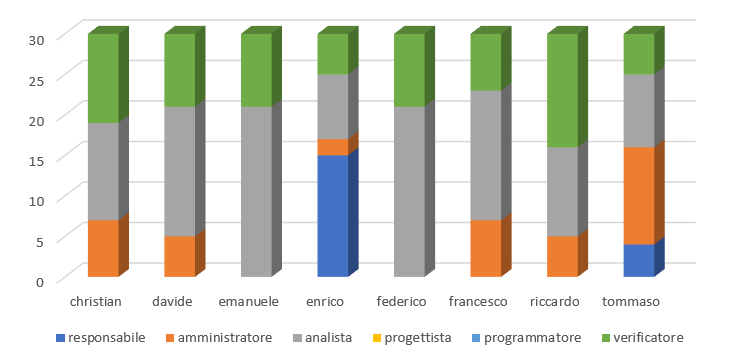
\includegraphics[scale=2.35]{sezioni/Istogrammi/IstogrammaAnalisi.png}
	
\end{figure}

\clearpage
\subsubsection{Costo Risultante}
La seguente tabella rappresenta per ogni ruolo le ore totali investite e il corrispondente costo in euro:
{
\rowcolors{2}{grigetto}{white}
\renewcommand{\arraystretch}{2}
\begin{table}[h]
\centering
\caption{Tabella del costo risultante di Analisi}
\begin{longtable}{ C{3cm} C{2cm} C{4cm}}
\rowcolor{darkblue}
	\textcolor{white}{\textbf{Ruolo}} & 
	\textcolor{white}{\textbf{Totale ore}} & 
	\textcolor{white}{\textbf{Costo ruolo in euro}}\\	
\endhead

        Responsabile & 19 & 570\\
        Amministratore & 38 & 760\\
        Analista & 114 & 2850 \\
        Progettista & 0 & 0 \\
        Programmatore & 0 & 0 \\
        Verificatore & 69 & 1035 \\
        \textbf{Totale} & 240 & 5215 \\
		
	\end{longtable}
\end{table}
}


La quantità di ore totali per ciascun ruolo viene rappresentata nel seguente areogramma:
\begin{figure}[h]
\centering
	\caption{Suddivisione ore per ruolo della fase di Analisi}
	
	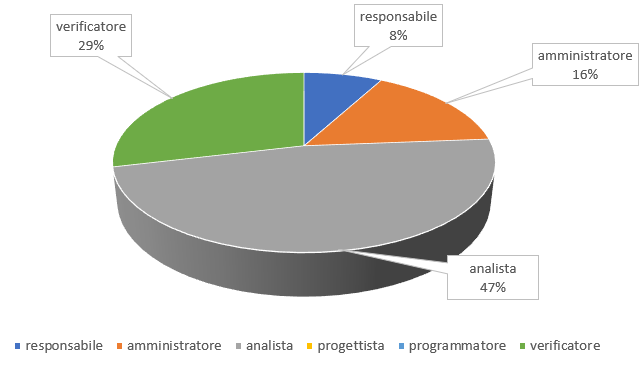
\includegraphics[scale=2.85]{sezioni/Aerogrammi/AerogrammaAnalisi.png}
\end{figure}
\clearpage

\subsection{Progettazione Architetturale}

\subsubsection{Divisione Oraria}
La seguente tabella rappresenta la distribuzione oraria dei ruoli per ogni componente del gruppo:
{
\rowcolors{2}{grigetto}{white}
\renewcommand{\arraystretch}{2}
\begin{table}[h]
\caption{Tabella della divisione oraria della Progettazione Architetturale}
\begin{longtable}{ C{5cm} C{1cm} C{1cm} C{1cm} C{1cm} C{1cm} C{1cm} C{3cm}}
\rowcolor{darkblue}
	\textcolor{white}{\textbf{Nome membro del gruppo}} & 
	\textcolor{white}{\textbf{RE}} & 
	\textcolor{white}{\textbf{AM}} & 
	\textcolor{white}{\textbf{AN}} & 
	\textcolor{white}{\textbf{PT}} & 
	\textcolor{white}{\textbf{PR}} & 
	\textcolor{white}{\textbf{VE}} & 
	\textcolor{white}{\textbf{Ore complessive}}\\	
	\endhead
        
    \MC{} & 5 & & & 14 & 10 & 4 & 33\\
    \LD{} & 8 & & & 18 & & 7 & 33 \\
    \CE{} & & 8 & & 10 & 5 & 6 & 29 \\
    \SE{} & & 10 & 6 & 10 & & 6 & 32 \\
    \PF{} & & 6 & & 5 & 7 & 13 &  31\\
    \DF{} & & & 13 & 5 & 7 & 6 & 31 \\
    \BR{} & 6 & & & & 17 & 8 & 31\\
   \AT{} & & & 8 & 7 & & 16 & 31\\
	\textbf{Ore totali ruolo} & 19 & 24 & 27 & 69 & 46 & 66 & 251\\
		
	\end{longtable}
\end{table}
}

La suddivisione delle ore svolte da ciascun componente del gruppo per ogni ruolo viene rappresentata nel seguente istogramma:

\begin{figure}[h!]
	\centering
	\caption{Disposizione ore per ruolo di ciascun componente della fase di Progettazione Architetturale}
	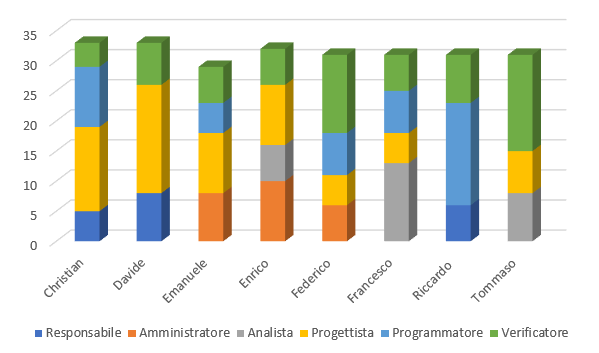
\includegraphics[scale=3]{sezioni/Istogrammi/IstogrammaProgettArchitetturale.png}
\end{figure}


\subsubsection{Costo Risultante}
La seguente tabella rappresenta per ogni ruolo le ore totali investite e il corrispondente costo in euro:
{
\rowcolors{2}{grigetto}{white}
\renewcommand{\arraystretch}{2}
\centering
\begin{table}[h]
\caption{Tabella del costo risultante della Progettazione Architetturale}
\begin{longtable}{ C{3cm} C{2cm} C{4cm}}
\rowcolor{darkblue}
	\textcolor{white}{\textbf{Ruolo}} & 
	\textcolor{white}{\textbf{Totale ore}} & 
	\textcolor{white}{\textbf{Costo ruolo in euro}}\\	
\endhead
        
        Responsabile & 19 & 570 \\
        Amministratore & 24 & 480 \\
        Analista & 27 & 675 \\
        Progettista & 69 & 1518 \\
        Programmatore & 46 & 690 \\
        Verificatore & 66 & 990 \\
        \textbf{Totale} & 251 & 4923 \\	
        	
	\end{longtable}
\end{table}
}

La suddivisione della quantità di ore totali per ciascun ruolo viene rappresentata nel seguente areogramma:

\begin{figure}[h]
	\centering
	\caption{Suddivisione ore per ruolo della fase di Progettazione Architetturale}
	
	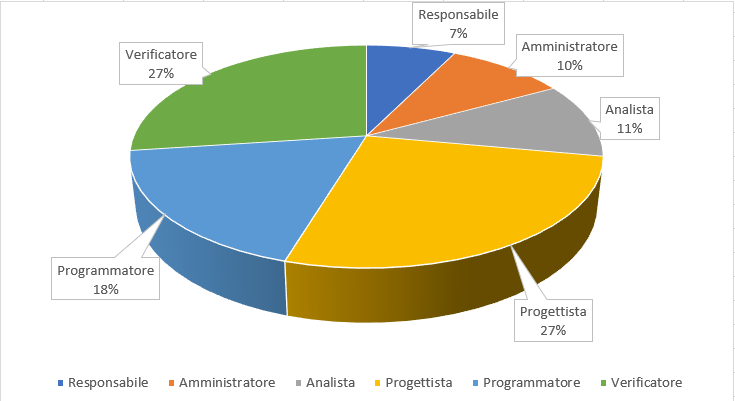
\includegraphics[scale=1.9]{sezioni/Aerogrammi/AerogrammaProgettArchitetturale.png}
\end{figure}

\clearpage
\subsection{Progettazione di dettaglio e codifica}

\subsubsection{Divisione Oraria}
La seguente tabella rappresenta la distribuzione oraria dei ruoli per ogni componente del gruppo:
{
	\rowcolors{2}{grigetto}{white}
	\renewcommand{\arraystretch}{2}
	\begin{table}[h]
	\caption{Tabella della divisione oraria della Progettazione di Dettaglio e Codifica}
	
\begin{longtable}{ C{5cm} C{1cm} C{1cm} C{1cm} C{1cm} C{1cm} C{1cm} C{3cm}}
\rowcolor{darkblue}
	\textcolor{white}{\textbf{Nome membro del gruppo}} & 
	\textcolor{white}{\textbf{RE}} & 
	\textcolor{white}{\textbf{AM}} & 
	\textcolor{white}{\textbf{AN}} & 
	\textcolor{white}{\textbf{PT}} & 
	\textcolor{white}{\textbf{PR}} & 
	\textcolor{white}{\textbf{VE}} & 
	\textcolor{white}{\textbf{Ore complessive}}\\
\endhead	
        
        \MC{} & & 10 & & 12 & 15 & 10 & 47\\
        \LD{} & 6 & & & 10 & 15 & 16 & 47\\
        \CE{} & & 5 & & 13 & 16 & 13 & 47 \\
        \SE{} & & 4 & & 11 & 18 & 14 & 47\\
        \PF{} & & 8 & & 8 & 19 & 12 & 47\\
        \DF{} & 10 & & & 7 & 17 & 13 & 47\\
        \BR{} & & 3 & & 12 & 19 & 13 & 47\\
       \AT{} & 10 & & & 10 & 17 & 10 & 47 \\
        \textbf{Ore totali ruolo} & 26 & 30 & & 83 & 136 & 101 & 376\\
		
	\end{longtable}
\end{table}
}
\newline
La suddivisione di quante ore, ciascun componente del gruppo, ha svolto per ogni ruolo viene rappresentata nel seguente istogramma:



\begin{figure}[h!]
\centering
\caption{Disposizione ore per ruolo di ciascun componente della fase di Progettazione di Dettaglio e Codifica}
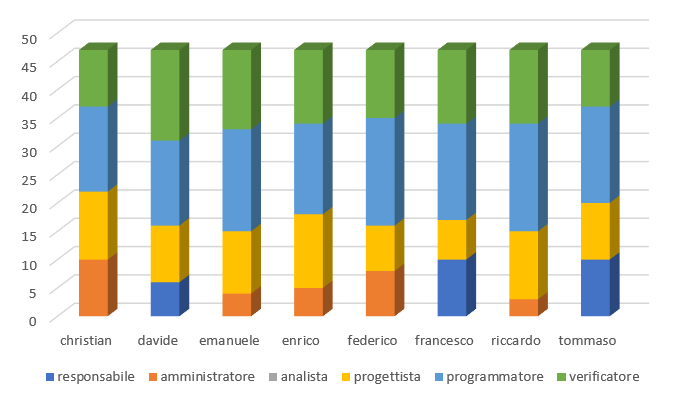
\includegraphics[scale=2.5]{sezioni/Istogrammi/IstogrammaDiDettaglio.png}
\end{figure}

\subsubsection{Costo Risultante}
La seguente tabella rappresenta, per ruolo, le ore totali investite e il corrispondente costo in euro:
{
\rowcolors{2}{grigetto}{white}
\renewcommand{\arraystretch}{2}
\begin{table}[h]
\centering
\caption{Tabella del costo risultante della Programmazione di Dettaglio e Codifica}
\begin{longtable}{ C{3cm} C{2cm} C{4cm}}
\rowcolor{darkblue}
	\textcolor{white}{\textbf{Ruolo}} & 
	\textcolor{white}{\textbf{Totale ore}} & 
	\textcolor{white}{\textbf{Costo ruolo in euro}}\\	
\endhead
        
        Responsabile & 26 & 780 \\
        Amministratore & 30 & 600 \\
        Analista & 0 & 0 \\
        Progettista & 83 & 1826 \\
        Programmatore & 136 & 2040 \\
        Verificatore & 101 & 1515\\
        \textbf{Totale} & 376 & 6761 \\
		
	\end{longtable}
\end{table}
}

La suddivisione della quantità di ore totali per ciascun ruolo viene rappresentata nel seguente areogramma:

\begin{figure}[h]
	\centering
	\caption{Suddivisione ore per ruolo della fase di Progettazione di Dettaglio e Codifica}
	
	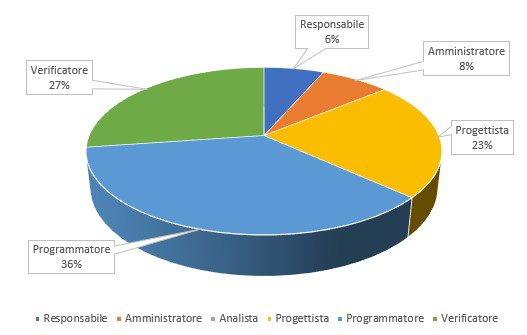
\includegraphics[scale=2.8]{sezioni/Aerogrammi/AerogrammaDiDettaglio.png}
\end{figure}

\clearpage
\subsection{Validazione e Collaudo}

\subsubsection{Divisione Oraria}
La seguente tabella rappresenta la distribuzione oraria dei ruoli per ogni componente del gruppo:
{
	\rowcolors{2}{grigetto}{white}
	\renewcommand{\arraystretch}{2}
	\begin{table}[h]
		\caption{Tabella della divisione oraria di Validazione e Collaudo}

	\begin{longtable}{ C{5cm} C{1cm} C{1cm} C{1cm} C{1cm} C{1cm} C{1cm} C{3cm}}
		\rowcolor{darkblue}
		\textcolor{white}{\textbf{Nome membro del gruppo}} & \textcolor{white}{\textbf{RE}} & \textcolor{white}{\textbf{AM}} & \textcolor{white}{\textbf{AN}} & \textcolor{white}{\textbf{PT}} & \textcolor{white}{\textbf{PR}} & \textcolor{white}{\textbf{VE}} & \textcolor{white}{\textbf{Ore complessive}}\\	
        
        \MC{} & & & 7 & & 4 & 8 & 19\\
        \LD{} & & 4 & & 5 & & 10 & 19\\
        \CE{} & 5 & & & & 6 & 12 & 23\\ 
        \SE{} & & & & 6 & 5 & 9 & 20 \\
        \PF{} & 6 & & & & 7 & 8 & 21\\
        \DF{} & & 6 & & & 9 & 6 & 21\\
        \BR{} & & 5 & & & 6 & 10 & 21\\
       \AT{} & & & 4 & 10 & & 7 & 21\\
        \textbf{Ore totali ruolo} & 11 & 15 & 11 & 21 & 37 & 70 & 165\\
		
	\end{longtable}
\end{table}
}


La suddivisione delle ore svolte da ciascun componente del gruppo per ogni ruolo viene rappresentata nel seguente istogramma:

\begin{figure}[h!]
	\centering
	\caption{Disposizione ore per ruolo di ciascun componente della fase di Validazione e Collaudo}
	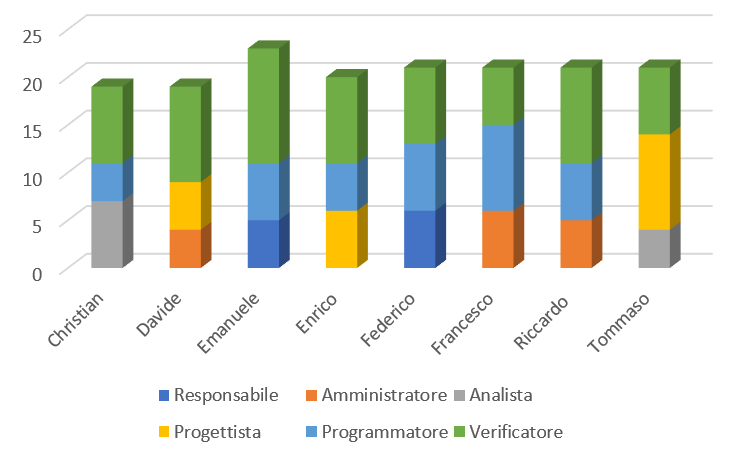
\includegraphics[scale=2.5]{sezioni/Istogrammi/IstogrammaValidazione.png}
\end{figure}

\subsubsection{Costo Risultante}
La seguente tabella rappresenta rappresenta per ogni ruolo le ore totali investite e il corrispondente costo in euro:
{
	\rowcolors{2}{grigetto}{white}
	\renewcommand{\arraystretch}{2}
\begin{table}[h!]
	\caption{Tabella del costo risultante di Validazione e Collaudo}
	\begin{longtable}	{ C{3cm} C{2cm} C{4cm}}

		\rowcolor{darkblue}
		\textcolor{white}{\textbf{Ruolo}} & \textcolor{white}{\textbf{Totale ore}} & \textcolor{white}{\textbf{Costo ruolo in euro}}\\	
        
        Responsabile & 11 & 330\\
        Amministratore & 15 & 300 \\
        Analista & 11 & 275\\
        Progettista & 21 & 462\\
        Programmatore & 37 & 555\\
        Verificatore & 70 & 1050\\
        \textbf{Totale} & 169 & 2972\
	
	\end{longtable}
\end{table}
	
}

La suddivisione della quantità di ore totali per ciascun ruolo viene rappresentata nel seguente areogramma:

\begin{figure}[h]
	\centering
	\caption{Suddivisione ore per ruolo della fase di Validazione e Collaudo}
	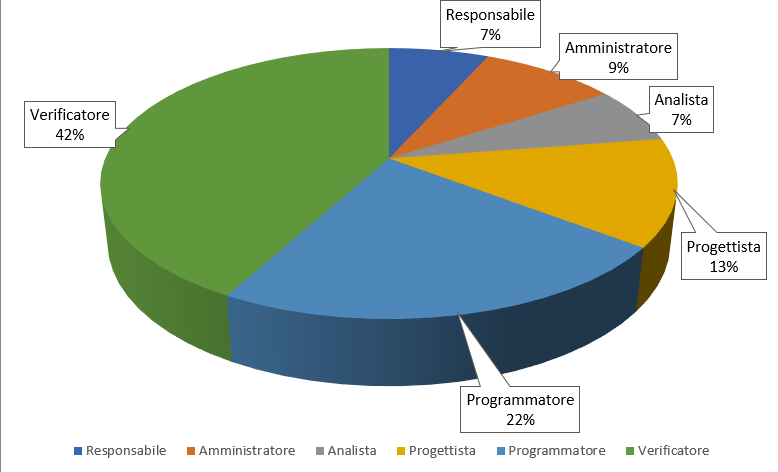
\includegraphics[scale=2.5]{sezioni/Aerogrammi/AerogrammaValidazione.png}
\end{figure}


\clearpage
\subsection{Preventivo finale} 
Nel preventivo riportiamo la spesa totale che il committente dovrà affrontare, derivata dal totale delle ore rendicontate e preventivate nelle fasi di Progettazione Architetturale, Progettazione di Dettaglio e Codifica, Validazione e Collaudo.

\subsubsection{Divisione oraria complessiva} 
Nella seguente tabella viene mostrata la distribuzione oraria dei ruoli per ogni componente del gruppo:
{
	\rowcolors{2}{grigetto}{white}
	\renewcommand{\arraystretch}{2}
\begin{table}[h]
		\caption{Tabella della divisione oraria complessiva}

	\begin{longtable}{ C{5cm} C{1cm} C{1cm} C{1cm} C{1cm} C{1cm} C{1cm} C{3cm}}
		\rowcolor{darkblue}
		\textcolor{white}{\textbf{Nome membro del gruppo}} & \textcolor{white}{\textbf{RE}} & \textcolor{white}{\textbf{AM}} & \textcolor{white}{\textbf{AN}} & \textcolor{white}{\textbf{PT}} & \textcolor{white}{\textbf{PR}} & \textcolor{white}{\textbf{VE}} & \textcolor{white}{\textbf{Ore complessive}}\\	
        
        \MC{} & 5 & 10 & 7 & 26 & 29 & 22 & 99 \\
        \LD{} & 14 & 4 & & 33 & 15 & 33 & 99\\
        \CE{} & 5 & 13 & & 23 & 27 & 31 & 99 \\
        \SE{} & & 14 & 6 & 27 & 23 & 29 & 99\\
        \PF{} & 6 & 14 & & 13 & 33 & 33 & 99\\
        \DF{} & 10 & 6 & 13 & 12 & 33 & 25 & 99 \\
        \BR{} & 6 & 8 & & 12 & 42 & 31 & 99 \\
       \AT{} & 10 & & 12 & 27 & 17 & 33 & 99 \\
        \textbf{Ore totali ruolo} & 56 & 69 & 38 & 173 & 219 & 237 &  792 \\

	\end{longtable}
\end{table}
}
\subsubsection{Costo complessivo per ruolo}
Nella seguente tabella viene illustrato il monte ore risultante per ogni ruolo con il costo ad esso associato:
{
	\rowcolors{2}{grigetto}{white}
	\renewcommand{\arraystretch}{2}
\begin{table}[h]
	\caption{Tabella del costo complessivo per ruolo}
	\begin{longtable}{ C{3cm} C{2cm} C{4cm}}
		\rowcolor{darkblue}
		\textcolor{white}{\textbf{Ruolo}} & \textcolor{white}{\textbf{Totale ore}} & \textcolor{white}{\textbf{Costo ruolo in euro}}\\	
        
        Responsabile & 56 &  1680\\
        Amministratore & 69 & 1380 \\
        Analista & 38 & 950 \\
        Progettista & 173 & 3806 \\
        Programmatore & 219 & 3285 \\
        Verificatore & 237 & 3555 \\
        	
	\end{longtable}
\end{table}
}

\subsubsection{Costo complessivo}
Nella seguente tabella vengono riportati i costi complessivi delle varie fasi e infine l'importo proposto da \Gruppo{} per la realizzazione del progetto \NomeProgetto{}:\\
{
	\rowcolors{2}{grigetto}{white}
	\renewcommand{\arraystretch}{2}

	\begin{table}[h]
	\caption{Tabella del costo complessivo}
	\begin{longtable}{ C{5cm} C{5cm}}
		\rowcolor{darkblue}
		\textcolor{white}{\textbf{Fase}} & \textcolor{white}{\textbf{Costo Fase}}\\	
		
		Progettazione Architetturale & 4923 \\
		Progettazione di Dettaglio e Codifica & 6761 \\
		Validazione e Collaudo & 2972 \\
		\textbf{Totale} & 14656\\
		
	\end{longtable}
\end{table}
}




\clearpage
\section{Consuntivo}

Nel Consuntivo approfondiamo il bilancio effettivo della fase di Analisi, ovvero la differenza tra le ore preventivate e quelle effettive.

\subsection{Analisi dei Requisiti}

Il bilancio della fase di Analisi è negativo, ovvero il gruppo ha impiegato più ore di quelle anticipate, quindi il costo finale della fase di Analisi supera l'aspettaviva calcolata in precedenza.\\
La seguente tabella illustra la differenza oraria ed economica rilevata a posteriori.

\rowcolors{2}{grigetto}{white}
\renewcommand{\arraystretch}{2}
\centering
\begin{longtable}{ C{5cm} C{1cm} C{1cm} C{1cm} C{1cm} C{1cm} C{1cm} C{3cm}}
	\rowcolor{rossoep}
	\textcolor{white}{\textbf{Ruolo}} & \textcolor{white}{\textbf{Ore preventivate}} & \textcolor{white}{\textbf{Ore supplementari}} & \textcolor{white}{\textbf{Costo preventivato}} & \textcolor{white}{\textbf{Costo effettivo}} & \textcolor{white}{\textbf{Differenza di costo}}\\	
	
	Responsabile & & & & & \\
	Amministratore & & & & & \\
	Analista & & & & & \\
	Progettista & & & & & \\
	Programmatore & & & & & \\
	Verificatore & & & & & \\
	\textbf{Totale} & & & & & & \\
	
\end{longtable}
\clearpage
\section{Organigramma}
\subsection{Redazione}
{
	\rowcolors{2}{grigetto}{white}
	\renewcommand{\arraystretch}{2}
	\begin{longtable}{ C{5cm} C{4cm} C{5cm} }
		\rowcolor{rossoep}
		\textcolor{white}{\textbf{Nome}} & \textcolor{white}{\textbf{Data di redazione}} & \textcolor{white}{\textbf{Firma}}\\	\endhead
        
        Davide Lazzaro & 2020-01-07 &   \\
        Enrico Salmaso & 2020-01-07 &   \\
        		
	\end{longtable}
}

\subsection{Approvazione}
{
	\rowcolors{2}{grigetto}{white}
	\renewcommand{\arraystretch}{2}
	\centering
	\begin{longtable}{ C{5cm} C{4cm} C{5cm} }
		\rowcolor{rossoep}
		\textcolor{white}{\textbf{Nome}} & \textcolor{white}{\textbf{Data di Approvazione}} & \textcolor{white}{\textbf{Firma}}\\	\endhead
		
		
		Enrico Salmaso & 2020-01-10 &  \\
		Tullio Vardanega &  & \\
		Riccardo Cardin & &  \\
		
	\end{longtable}
}

\subsection{Accettazione dei componenti}
{
	\rowcolors{2}{grigetto}{white}
	\renewcommand{\arraystretch}{2}
	\begin{longtable}{ C{5cm} C{4cm} C{5cm} }
		\rowcolor{rossoep}
		\textcolor{white}{\textbf{Nome}} & \textcolor{white}{\textbf{Data di Accettazione}} & \textcolor{white}{\textbf{Firma}}\\	\endhead
		
		
		Christian Mattei & & \\
		Davide Lazzaro & & \\
		Emanuele Cisotto & & \\
		Enrico Salmaso & &  \\
		Federico Perin & & \\
		Francesco Drago & &  \\
		Riccardo Baratin & &  \\
		Tommaso Azzalin & &  \\
		
		
	\end{longtable}
}

\subsection{Componenti}
{
	\rowcolors{2}{grigetto}{white}
	\renewcommand{\arraystretch}{2}
	\begin{longtable}{ C{4cm} C{2cm} C{8cm} }
		\rowcolor{rossoep}
		\textcolor{white}{\textbf{Nome}} & \textcolor{white}{\textbf{Matricola}} & \textcolor{white}{\textbf{Indirizzo di posta elettronica}}\\\endhead	
		
		Christian Mattei & 1121305 & christian.mattei@studenti.unipd.it \\
		Davide Lazzaro & 1162190 & davidemaria.lazzaro@studenti.unipd.it\\
		Emanuele Cisotto & 1161514 & emanuele.cisotto@studenti.unipd.it\\
		Enrico Salmaso & 1166175 & enrico.salmaso.2@studenti.unipd.it \\
		Federico Perin & 1170747 & federico.perin.1@studenti.unipd.it \\
		Francesco Drago & 1146928 & francesco.drago.1@studenti.unipd.it \\
		Riccardo Baratin & 1148142 & riccardo.baratin@studenti.unipd.it \\
		Tommaso Azzalin & 1169740 & tommaso.azzalin@studenti.unipd.it \\
		
		
	\end{longtable}
}
\clearpage

\end{document}